\documentclass[a4paper,12pt]{extarticle}
\usepackage{mathptmx}
% Language setting
% Replace `english' with e.g. `spanish' to change the document language
\usepackage[utf8]{inputenc}

\usepackage{cite}
\usepackage{amsmath,amssymb,amsfonts}
\usepackage{algorithmic}
\usepackage{graphicx}
\usepackage{textcomp}
%\usepackage{xcolor}
\usepackage{booktabs}
\usepackage{float}
\usepackage{multicol}
\usepackage[absolute,overlay]{textpos}
\usepackage{makecell}
\usepackage[colorlinks=true, allcolors=black]{hyperref}
\usepackage{subcaption}
\usepackage[table]{xcolor}
\usepackage{multirow}
\setlength{\arrayrulewidth}{1mm}
\setlength{\tabcolsep}{18pt}
\renewcommand{\arraystretch}{2}
\newcolumntype{s}{>{} p{3cm}}



\usepackage{graphicx} % Required for inserting images
\usepackage{tikz}
\usetikzlibrary{shapes.geometric, arrows}

% Set page size and margins
% Replace `letterpaper' with`a4paper' for UK/EU standard size
\usepackage[letterpaper,top=2cm,bottom=2cm,left=2.5cm,right=2.5cm,marginparwidth=1.75cm]{geometry}

% Useful packages
\usepackage{amsmath}
\usepackage{graphicx}
\newpage



\makeatletter
\renewenvironment{abstract}{%
    \if@twocolumn
      \section*{\abstractname}%
    \else %% <- here I've removed \small
      \begin{center}%
        {\bfseries \Large\abstractname\vspace{\z@}}%  %% <- here I've added \Large
      \end{center}%
      \quotation
    \fi}
    {\if@twocolumn\else\endquotation\fi}
\makeatother
\bibliographystyle{IEEEtran}
\bigskip
\bigskip
\bigskip
\bigskip
\bigskip
\bigskip
\bigskip
\bigskip
\bigskip
\title{\textbf{Classification of Brain Tumors using Deep Learning Method}}


\date{}
\begin{document}
\maketitle
\vspace{-2em}



\centerline{\textbf{CSE 4120 Technical Writing and Seminar lab}}


\begin{figure}[H]
\centerline{
\includegraphics[
  height=3.5cm]{figure/logo.png}}
\label{fig:dat}
\end{figure}
\bigskip
\bigskip
\bigskip

\centerline{\textbf{Submitted To:}}
\centerline{\textbf{Dr. K. M. Azharul Hasan}}
\centerline{\textbf{Professor}}
\centerline{\textbf{Sunanda Das}}
\centerline{\textbf{Assistant Professor}}

\bigskip
\bigskip

\bigskip

\bigskip
\bigskip


\centerline{\textbf{Submitted by:}}
\centerline{\textbf{Shrabanti Debnath Urmi}}
\centerline{\textbf{Roll: 1907094}}
\centerline{\textbf{Computer Science \& Engineering}}
\centerline{\textbf{Khulna University Of Engineering \& Technology}}
\pagebreak

\tableofcontents
\clearpage

\listoffigures
\listoftables
\clearpage
\begin{abstract}
\normalsize
To classify brain tumors from MRI scans, recent research has focused on using deep learning techniques. One study developed a model to predict the methylation status of the MGMT promoter in glioblastoma. Another study utilized YOLOv5 and YOLOv7 architectures to segment and classify brain tumors.A third study used transfer learning with a pre-trained GoogLeNet model to classify tumors into categories. These approaches combine deep learning and IoT-enabled systems to improve brain tumor diagnosis and patient care.
\end{abstract}
\pagebreak

\section{Introduction}

A brain tumor is a severe disease. In 2021, there will be around 84,000 new cases of primary brain tumors diagnosed, and 18,600 new cases of malignant brain tumors (brain cancer) would likely result in deaths.[8] Magnetic Resonance Imaging (MRI) is the most effective method for detecting brain malignancies. Brain tumors\cite{shen2017deep} have the potential to have permanent and life-altering physical, cognitive, and psychological effects on a patient, more so than any other malignancy. For this reason, the best treatment plan and a quicker diagnosis should be developed in order to maximize the patients' chances of survival. In picture classification and segmentation tasks, neural networks have demonstrated astounding accuracy.

Glioblastoma is one of the most aggressive forms of the disease. We have used deep learning algorithms to detect brain tumors and it has showed result of precise diagnoses. The success of chemotherapy depends on how we understand the methylation state of O6-Methylguanine-DNA Methyltransferase (MGMT)\cite{litjens2017survey} in malignancies. RSNA and MICCAI use sophisticated imaging methods to improve diagnosis and treatment planning. Deep learning with convolutional neural networks (CNNs), has been able to automatically recognize and classify brain tumors which can lead us to improved patient care. YOLOv5 and YOLOv7 are classification techniques and they help improving accuracy and speed of the method. Despite progress, there are still issues in development for this area of healthcare.
 


\section{Problem Statement}

\begin{itemize}

    \item To build deep learning models to identify and categorize brain tumour on MRI pictures.
    \item To increase accuracy and practically make these diagnostic procedures faster
    \item To detect brain tumors in the early stages.
    \item To focus on issues like computational complexity for near real-time applications.
\end{itemize}

\section{Review of Literature}

\begin{itemize}
    \item Deep learning algorithms, particularly CNNs, have shown promising results in accurately detecting brain tumors using MRI images, CT scans, and EEG data.
    \item Various deep learning models and techniques, including CNNs, RNNs, AEs, transfer learning, and hybrid algorithms, have been explored for brain tumor detection and classification.
    \item BrainMRNet achieved 96\% accuracy using an end-to-end CNN model on MR images.
    \item Patch-based DNN achieved a high Dice Similarity Coefficient of 99.8\% on BraTS 2013 dataset for brain tumor classification.
    \item Transfer learning techniques, such as using pre-trained CNNs like ResNet50-v2, have resulted in impressive accuracies exceeding 99%.
    \item Faster R-CNN and CNN architectures achieved average precision rates of 77.60\% and 96.56\%, respectively, for brain tumor detection and classification.
\end{itemize}

        

\section{Methodology of Proposed System}
\subsection{Deep Learning Approach for Radiogenomic Classification of Brain Tumor}
\subsubsection{Flow Chart of Radiogenomic Classification of Brain Tumor}
\begin{figure}[H] % Adjust placement specifier as needed
    \centering
    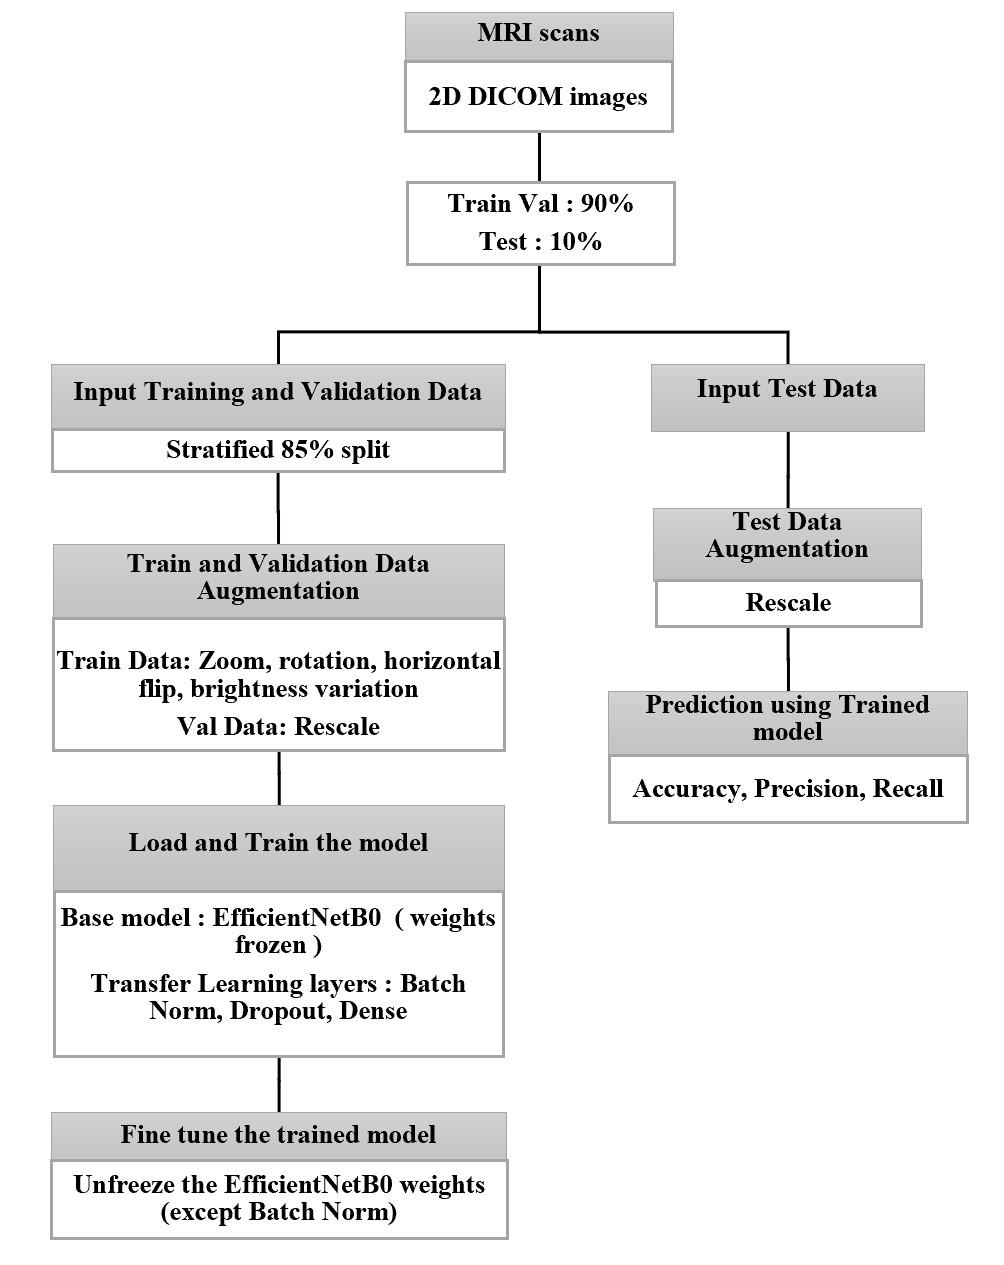
\includegraphics[width=\linewidth, height=13.7cm, keepaspectratio]{figure/paper1.png}
    \caption{learning framework}
    \label{fig:learning framework}
\end{figure}
\begin{itemize}
    \item Data Loading: Loading the MRI dataset and splitting it into training, validation, and test sets.
    \item Data Augmentation: Applying techniques such as rotation, flipping, and brightness adjustment to increase the diversity of the training data.
    \item Model Initialization: Initializing the model using EfficientNetB0 with pre-trained\cite{kamnitsas2017efficient} weights from ImageNet.
    \item Transfer Learning: Training the added layers on the augmented dataset while keeping the pre-trained layers frozen.
    \item Fine-Tuning: Unfreezing all model layers and further train the entire model on the augmented dataset with a reduced learning rate.
    \item Evaluation: Evaluating the model's performance using the validation set, computing metrics such as accuracy, loss, precision, recall, and F1-score.
    \item Prediction: Using the trained model to predict the methylation status of the MGMT promoter on unseen test data to assess its generalization performance.
\end{itemize}




\subsubsection{Four Modalities of Imaging}
\begin{figure}[H]
    \centering
    \begin{subfigure}[b]{0.24\linewidth}
        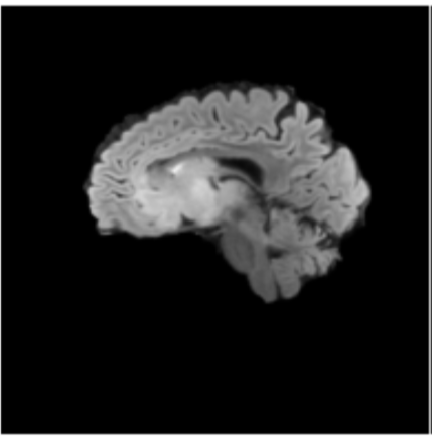
\includegraphics[width=\linewidth]{figure/flair.png}
        \caption{Flair}
        \label{fig:img1}
    \end{subfigure}
    \begin{subfigure}[b]{0.24\linewidth}
        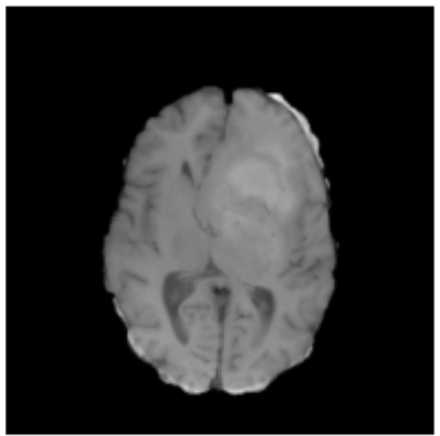
\includegraphics[width=\linewidth]{figure/t1w.png}
        \caption{T1w}
        \label{fig:img2}
    \end{subfigure}
    \begin{subfigure}[b]{0.24\linewidth}
        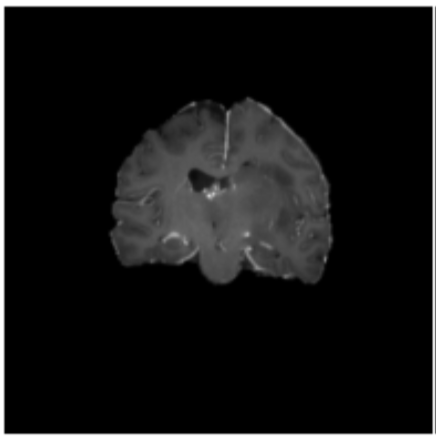
\includegraphics[width=\linewidth]{figure/t1gd.png}
        \caption{T1Gd}
        \label{fig:img3}
    \end{subfigure}
    \begin{subfigure}[b]{0.24\linewidth}
        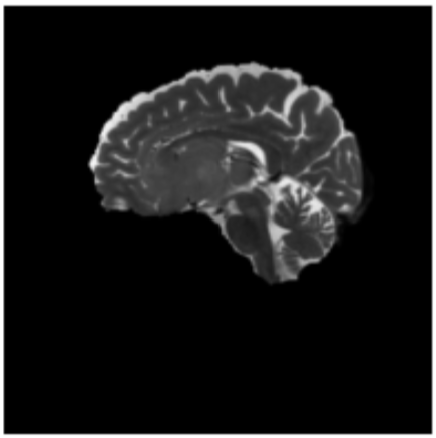
\includegraphics[width=\linewidth]{figure/t2w.png}
        \caption{T2w}
        \label{fig:img4}
    \end{subfigure}
    \caption{Scans representing four modalities of imaging}
    \label{fig:four_modalities}
\end{figure}


\newpage
\subsection{Automated Brain Tumor Segmentation
and Classification in MRI Using
YOLO-Based Deep Learning}
\subsubsection{Flow Chart of YOLO-based Brain Tumor Segmentation and Classification}
\begin{figure}[H] % Adjust placement specifier as needed
    \centering
    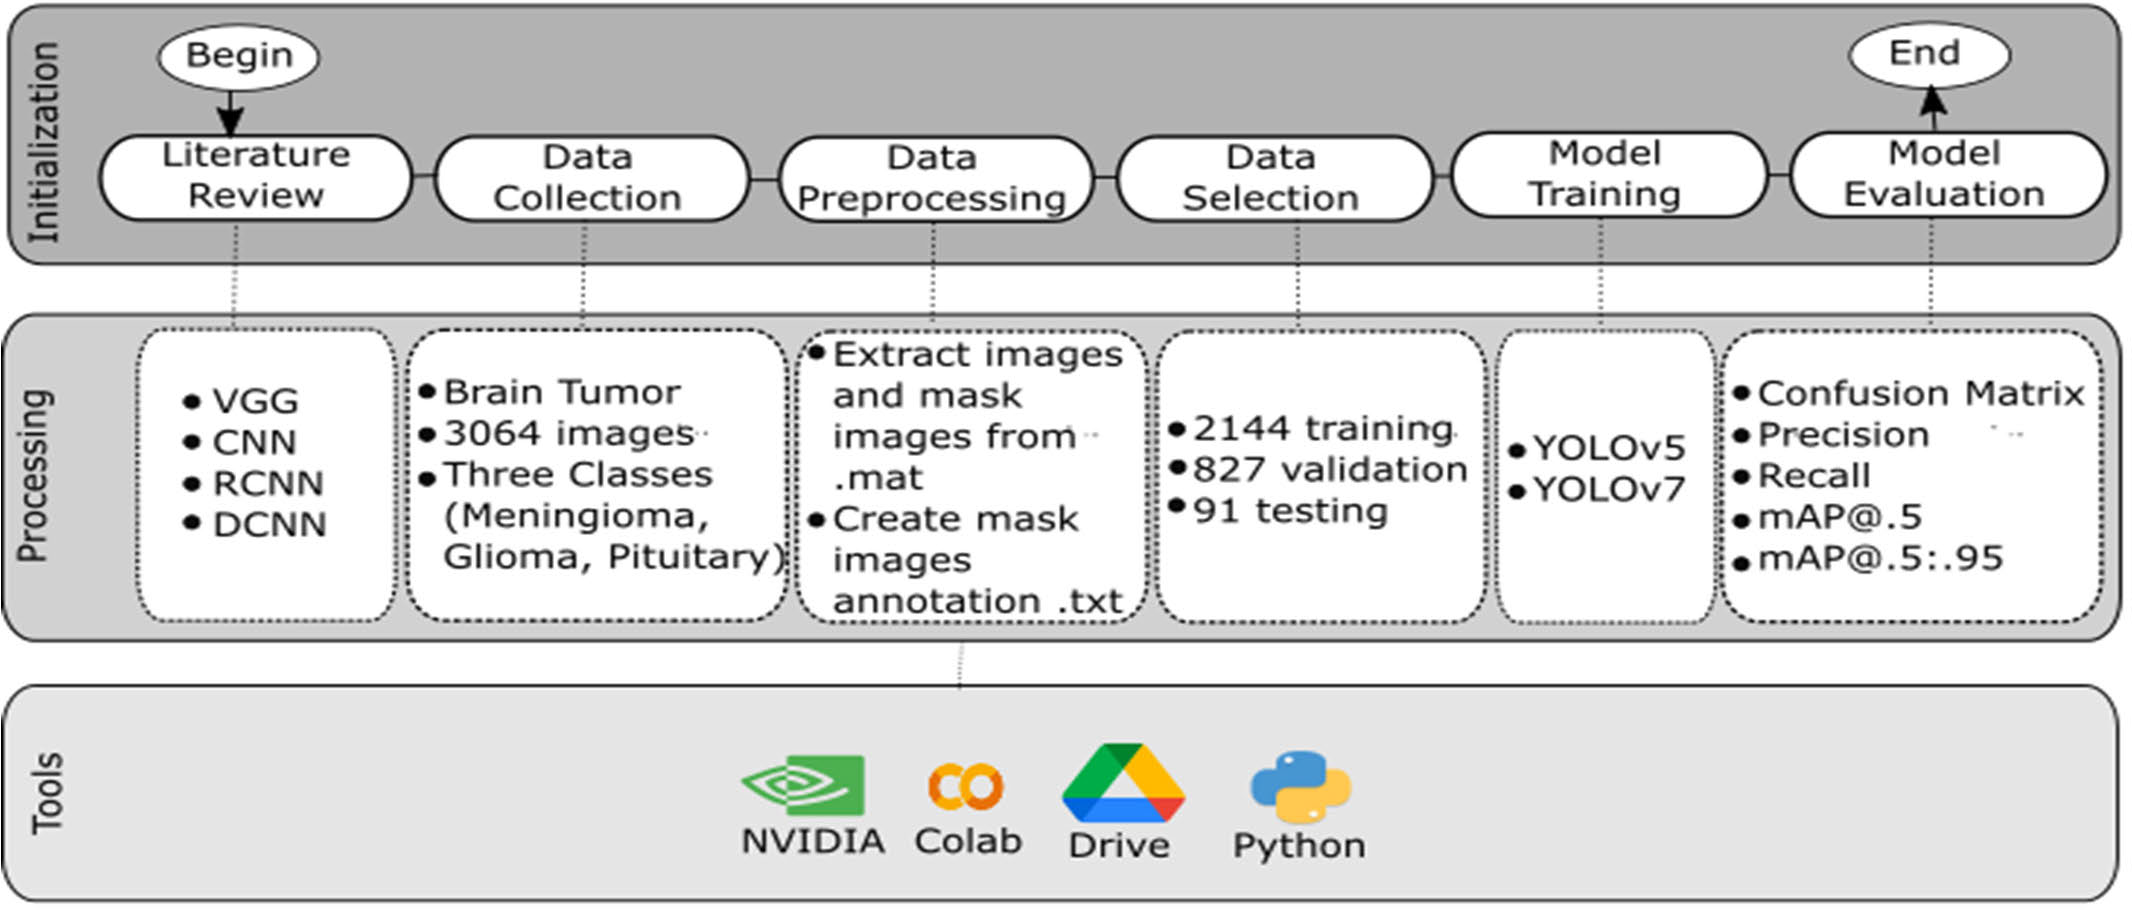
\includegraphics[width=\linewidth, height=13.7cm, keepaspectratio]{figure/yolo.png}
    \caption{YOLO-based Brain Tumor Segmentation and Classification Research Flow Diagram}
    \label{fig:YOLO-based Brain Tumor Segmentation and Classification Research Flow Block Diagram.}
\end{figure}
\subsubsection{Data Collection}
\textbf{Dataset}: 
\[ \text{Dataset} = \{\text{MRI images of brain tumors}\} \]
\textbf{Dataset Size}: 
\[ |\text{Dataset}| = 3064 \text{ images} \]
\textbf{Classes}: 
\[ \text{Classes} = \{\text{meningioma, glioma, pituitary}\} \]
\textbf{Class Proportions}:
\begin{itemize}
    \item Meningioma: \(23.11\% \)
    \item Glioma: \(30.35\% \)
    \item Pituitary: \(46.54\% \)
\end{itemize}

\subsubsection{Data Preprocessing}
\textbf{Conversion to PNG}: 
\[ \text{PreprocessedData} = \text{ConvertToPNG}(\text{Data}) \]
\textbf{Annotation using Masks}: 
\[ \text{AnnotatedData} = \text{AnnotateWithMasks}(\text{PreprocessedData}) \]

\subsubsection{Data Selection}
\textbf{Dataset Split}:
\begin{itemize}
    \item Training Set: \( \text{TrainSet} = 2144 \) images
    \item Validation Set: \( \text{ValidationSet} = 827 \) images
    \item Testing Set: \( \text{TestSet} = 91 \) images
\end{itemize}

\subsubsection{Model Training}
\textbf{1) YOLOv5 Model}
\begin{itemize}
    \item \textbf{Initialization}: 
    \[ \text{Model}_{\text{YOLOv5}} = \text{InitializeModel}(\text{Parameters}_{\text{YOLOv5}}) \]
    \item \textbf{Training}: 
    \[ \text{TrainedModel}_{\text{YOLOv5}} = \text{TrainModel}(\text{Model}_{\text{YOLOv5}}, \text{TrainSet}) \]
\end{itemize}

\textbf{2) YOLOv7 Model}
\begin{itemize}
    \item \textbf{Initialization}: 
    \[ \text{Model}_{\text{YOLOv7}} = \text{InitializeModel}(\text{Parameters}_{\text{YOLOv7}}) \]
    \item \textbf{Training}: 
    \[ \text{TrainedModel}_{\text{YOLOv7}} = \text{TrainModel}(\text{Model}_{\text{YOLOv7}}, \text{TrainSet}) \]
\end{itemize}

\subsubsection{Evaluation Parameters}
\textbf{Confusion Matrix}: Provides insights into model precision and inaccuracies. \\
\textbf{Loss Function}: 
\[ \text{Loss} = \text{l}_{\text{box}} + \text{l}_{\text{cls}} + \text{l}_{\text{obj}} \]
\textbf{Precision}: 
\[ \text{Precision} = \frac{TP}{TP + FP} \]
\textbf{Recall}: 
\[ \text{Recall} = \frac{TP}{TP + FN} \]
\textbf{Mean Average Precision (mAP)}: 
\[ \text{mAP} = \frac{1}{n} \sum_{k=1}^{n} \text{AP}_k \]
\textbf{F1-Confidence Curve}: Illustrates the correlation between F1 score and confidence threshold.

\newpage
\subsection{Brain Tumor Classification Using Fine-Tuned
GoogLeNet Features and Machine Learning
Algorithms: IoMT Enabled CAD System}
\subsubsection{Flow Chart of brain tumor classification using fine-tuned googlenet features}
\begin{figure}[H] % Adjust placement specifier as needed
    \centering
    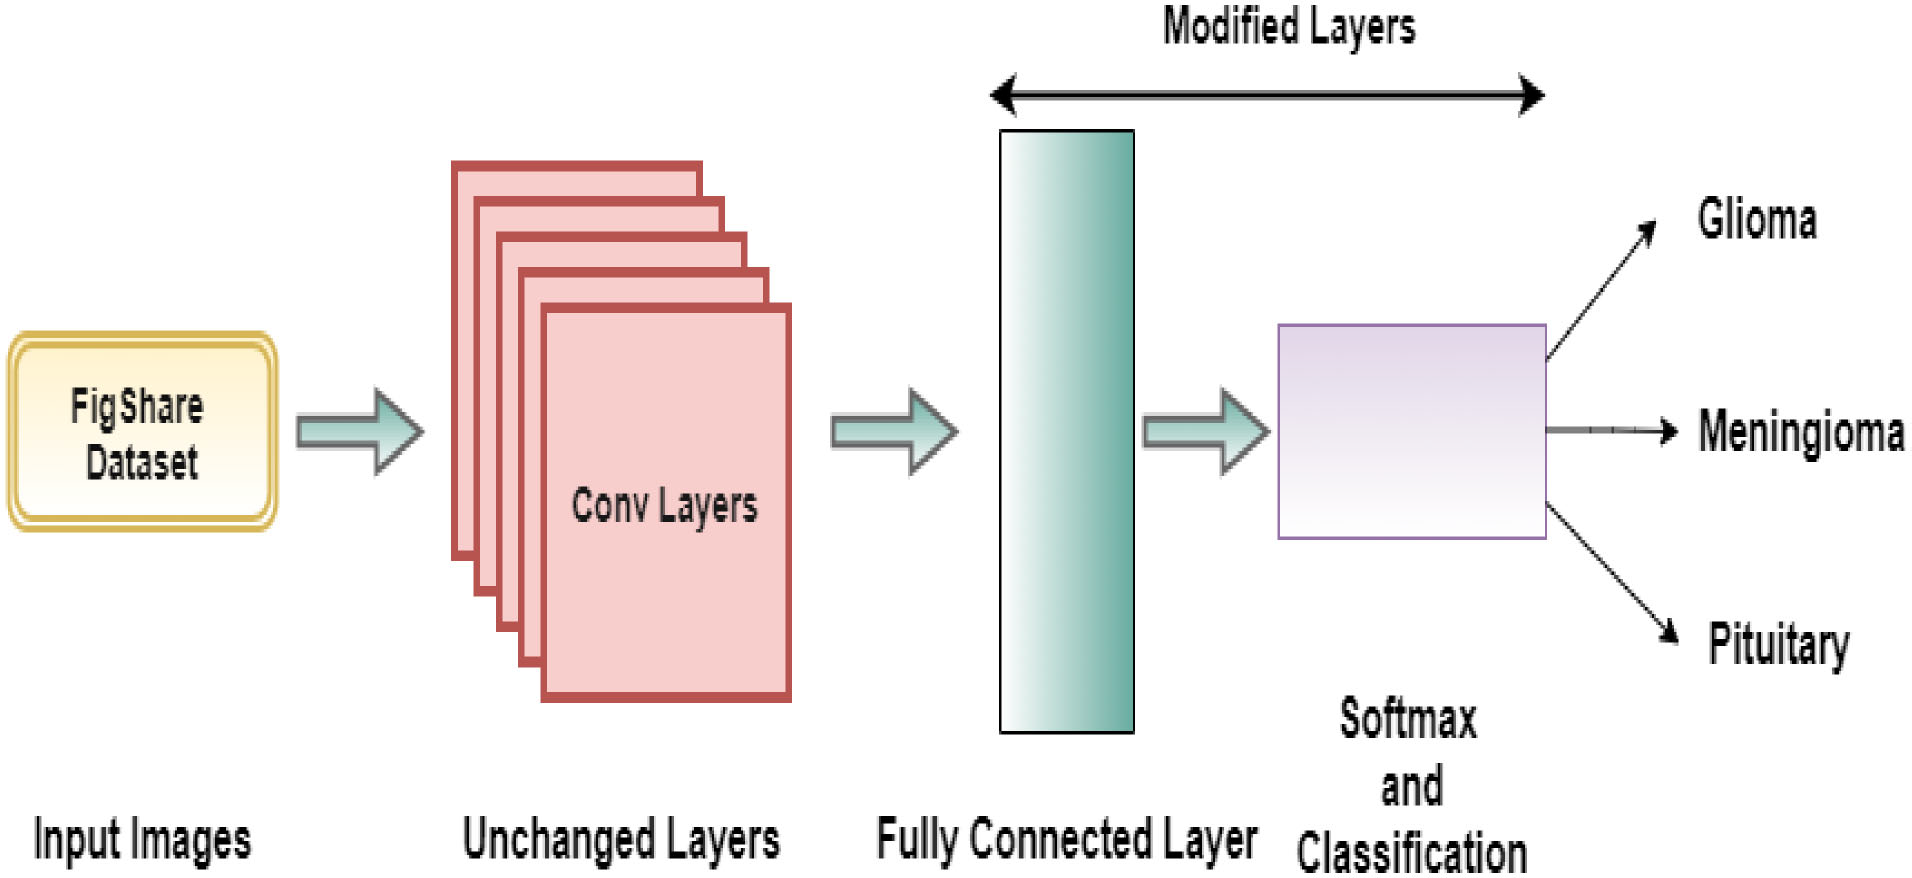
\includegraphics[width=\linewidth, height=13.7cm, keepaspectratio]{figure/archi.png}
    \caption{Architecture of classification using fine-tuned googlenet.}
    \label{fig:Architecture of classification using fine-tuned googlenet.}
\end{figure}
\subsubsection{Pre-Processing}
The intensity of MR images is normalized using min-max normalization:
\[ y_i = \frac{x_i - \text{min}(x)}{\text{max}(x) - \text{min}(x)} \]

The images are resized from \(512 \times 512\) to \(224 \times 224\) and converted to RGB.

\subsubsection{Training CNN}
CNNs are trained using backpropagation algorithm to minimize the cost function:
\[ C = -\frac{1}{n} \sum_{i=1}^{n} \ln(P(y_i|x_i)) \]

Weights are updated iteratively using the backpropagation algorithm.

\subsubsection{Transfer Learning and Fine-Tuned GoogLeNet}
GoogLeNet is fine-tuned for brain tumor classification.
The fully connected layer of GoogLeNet is replaced with a layer having output size 3.
Weights and biases are initialized and updated during training.
The modified GoogLeNet\cite{isensee2021nnU} architecture includes convolution layers followed by fully connected layers.
The output layer classifies tumors into three types using softmax function.


\begin{table}[H]
\centering
\caption{Result Analysis}
\label{tab:result_analysis}
\resizebox{\linewidth}{!}{%
\begin{tabular}{lccc}
\hline
\textbf{Paper} & \textbf{Accuracy (\%)} & \textbf{AUC} & \textbf{Fine-tuning Improvement (\%)} \\
\hline
Paper 1 & FLAIR: 64.20 & FLAIR: 0.5077 & FLAIR: +11.80 \\
 & T1-weighted: 71.92 & T1-weighted: 0.4443 & T1-weighted: +23.31 \\
 & T1wCE: 53.6 & T1wCE: 0.4945 & T1wCE: +6.87 \\
 & T2-weighted: 61.51 & T2-weighted: 0.4945 & T2-weighted: +7.54 \\
\hline
Paper 2 & Box Training Loss: YOLOv5-0.017893, YOLOv7-0.012063 & - & - \\
 & Segmentation Training Loss: YOLOv5-0.014582, YOLOv7-0.017295 & - & - \\
 & Object Training Loss: YOLOv5-0.005704, YOLOv7-0.00412 & - & - \\
 & Classification Training Loss: YOLOv5-0.000391, YOLOv7-0.000368 & - & - \\
\hline
Paper 3 & GoogLeNet + Softmax: 94.9\% & GoogLeNet + Softmax: 0.9979 & GoogLeNet + Softmax: - \\
 & GoogLeNet + SVM: 97.6\% & GoogLeNet + SVM: 0.9949 & GoogLeNet + SVM: +2.7\% \\
 & GoogLeNet + K-NN: 98.3\% & GoogLeNet + K-NN: 0.9937 & GoogLeNet + K-NN: +3.4\% \\
\hline
\end{tabular}%
}
\end{table}





\begin{figure}[H]
   
    \centering
    \begin{subfigure}[b]{0.2\textwidth}
        \centering
        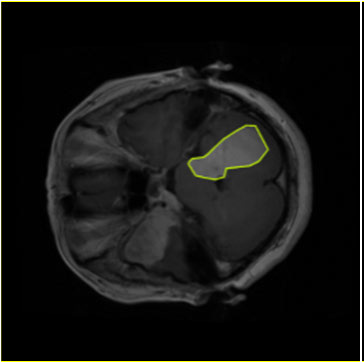
\includegraphics[width=\textwidth]{figure/1.png}
    \end{subfigure}
    \begin{subfigure}[b]{0.2\textwidth}
        \centering
        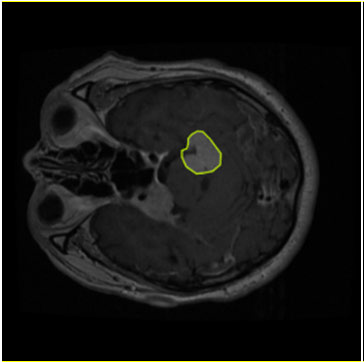
\includegraphics[width=\textwidth]{figure/2.png}
    \end{subfigure}
    \begin{subfigure}[b]{0.2\textwidth}
        \centering
        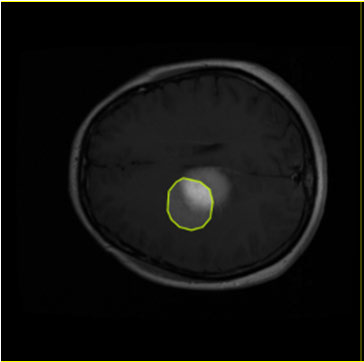
\includegraphics[width=\textwidth]{figure/3.png}
    \end{subfigure}
    \begin{subfigure}[b]{0.2\textwidth}
        \centering
        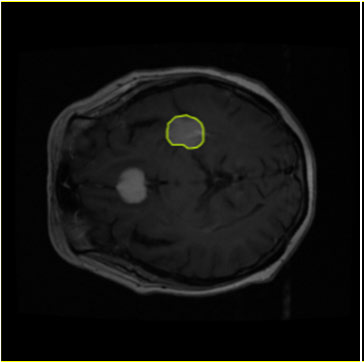
\includegraphics[width=\textwidth]{figure/4.png}
    \end{subfigure}
    \caption{Before tumor mask alignment (5.1)}
    \label{fig:before_alignment}
\end{figure}

\begin{figure}[H]
    \ContinuedFloat
    \centering
    \begin{subfigure}[b]{0.2\textwidth}
        \centering
        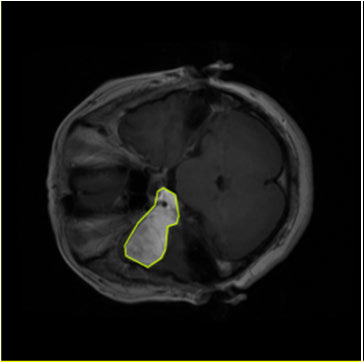
\includegraphics[width=\textwidth]{figure/5.png}
    \end{subfigure}
    \begin{subfigure}[b]{0.2\textwidth}
        \centering
        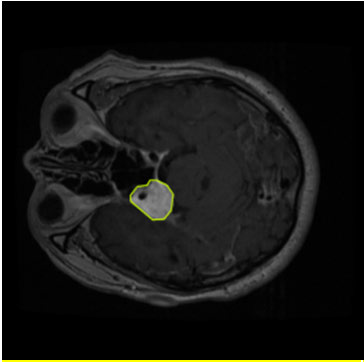
\includegraphics[width=\textwidth]{figure/6.png}
    \end{subfigure}
    \begin{subfigure}[b]{0.2\textwidth}
        \centering
        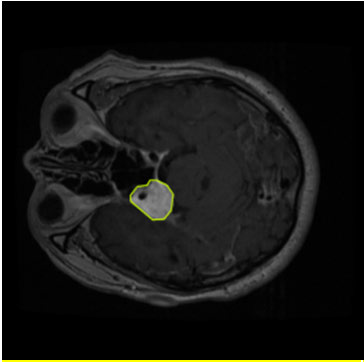
\includegraphics[width=\textwidth]{figure/7.png}
    \end{subfigure}
    \begin{subfigure}[b]{0.2\textwidth}
        \centering
        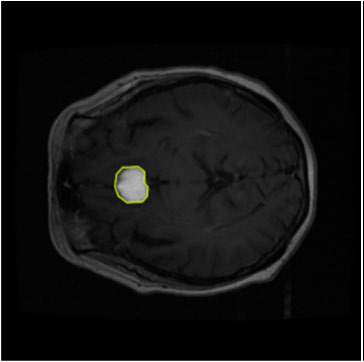
\includegraphics[width=\textwidth]{figure/8.png}
    \end{subfigure}
    \caption{After tumor mask alignment (5.2)}
    \label{fig:second_row}
\end{figure}



\newpage


\section{Recommendation}
\begin{itemize}
    \item It can as well be deduced from the paper that Paper 3 provides the most accurate result out of the three papers provided. Here's why:
    \subsubsection{Accuracy:}
     \begin{itemize}
         \item  In comparison, Paper 3 has the highest accuracy out of three papers in which the GoogLeNet model with the K-NN classifier are tested with an accuracy of 98.3. This is higher than what was reported in papers 1 and 2.
     \end{itemize}
      \subsubsection{AUC:}
      \begin{itemize}
         \item In the results presented by the authors in Paper 3, AUCs noted for all tumor types for each classifier (Softmax, SVM, and K-NN) are high, suggesting that the method does not fail to achieve good classification\cite{zhang2020dual} accuracy in distinguishing between the types of tumors.
     \end{itemize}
     \subsubsection{Fine-tuning Improvement:}
   \begin{itemize}
         \item The GoogLeNet model is fine tuned and Paper 3 shows that enhancement in accuracy is by far huge. This fine-tuning helps the mode to better capture the relevant cues from the MRI image, resulting in improved classification.
     \end{itemize}
\end{itemize}

\section{Findings}
\subsubsection{paper1}
\begin{itemize}
    \item  As pointed out in the report, they achieve higher accuracies after tuning up in comparison to the other models, though not as high as those obtained in Paper 3. Nonetheless, it is still useful to look at the available findings insofar helping to decide the possibility of transfer learning and fine-tuning utilizing MRI images and in the detection of brain tumor.
\end{itemize}
\subsubsection{paper2}
\begin{itemize}
    \item Here the primary focus of concern pays attention to the segmentation and classification of the brain tumor\cite{pereira2016brain} through the YOLO-based models. While the paper describes the notions of loss performance and precision, and other equal performances like recall and other performances, it offers lower reported accuracies\cite{isensee2021nnU} linked to the Paper 3. Anyway it may be useful for emerging more detailed knowledge regarding the methods of deep learning-application on the subject of the brain tumor segmentation.
\end{itemize}


\newpage
\section{Addressing Course outcomes and Program Out-
comes}
The analysis of these three papers has a relation with the educational outcomes as-
\begin{itemize}
    \item  Analyzing the papers, finding out the problems, finding out the key method-ologies of each paper, comparing the results of these three papers and recom-mending one, improves our problem analysis ability.

    \item  Adding proper citations and references improves our ethical principles. Be-cause adding citations will effectively help us to avoid plagiarism.
    \item Making presentation slides on the selected topic and presenting to the audience will develop presentation skills as well as communication skills which will help us in future to do individual work as well as teamwork.
\item  Writing report on the selected topic will significantly develop our analyzing power and our ability to summarize a topic.

\end{itemize}

\section{Addressing Complex Engineering Activities}
\begin{itemize}
    \item Every paper needs different input like research, technical, financial, and sometimes hardware input consisting of various instruments like sensors and trunk infrastructure.

\item All the papers raise certain issues: this is selecting the most appropriate method out of several, working on the practical application time constraints, and fine-tuning classifiers for maximum accuracy.






\end{itemize}

\section{Conclusion}
Thus, it is clear that the three papers as a whole contribute to the development of brain tumor detection and classification by employing methodologies as well as deeper learning. In general, each paper utilizes various techniques to achieve a common objective of enhancing the diagnostic outcomes for brain tumors utilizing MRI pictures. For the same, Paper 3 is truly significant as it presents a good result of fine-tuning GoogLeNet through small K-NN classifier, which can be further explored and analyzed. Papers 1 and 2, although reported slightly lower accuracy than papers 3 and 4, offers a good background on the applicability of transfer learning as well as YOLO techniques in tumor detection and segmentation. All together, these papers stress the importance of cooperation between other disciplines and constant work to create solutions for the engineering issues affecting society and environment.

\pagebreak


\bibliography{Reference}
\end{document}